\chapter{Theory}\label{ch:theory}
Here is the theory.

\begin{table}[]
\centering
\caption{The beginnings of the Golomb and Rice codes for a few parameter values. The midpoint ($\cdot$) separates the high-order (unary) part from the low-order (binary) part of the codewords. The codes can be extended to all values of $n\geq0$.}
\label{table:golomb-rice}
\begin{tabular}{rrrrr}
\multicolumn{1}{c}{Golomb}   & \multicolumn{1}{c}{$m=1$}   & \multicolumn{1}{c}{$m=2$}   & \multicolumn{1}{c}{$m=4$}   & \multicolumn{1}{c}{$m=8$}   \\
\multicolumn{1}{c}{Rice}     & \multicolumn{1}{c}{$k=0$}   & \multicolumn{1}{c}{$k=1$}   & \multicolumn{1}{c}{$k=2$}   & \multicolumn{1}{c}{$k=3$}   \\
\hline % --------------------------------------------------------------------------------------------------------------------------------------------
\multicolumn{1}{r|}{$n=0$}   & \textbf{0$\cdot$}           & \textbf{0$\cdot$0}          & \textbf{0$\cdot$00}         & \textbf{0$\cdot$000}        \\
\multicolumn{1}{r|}{      1} & \textbf{10$\cdot$}          & \textbf{0$\cdot$1}          & \textbf{0$\cdot$01}         & \textbf{0$\cdot$001}        \\
\multicolumn{1}{r|}{      2} & \textbf{110$\cdot$}         & \textbf{10$\cdot$0}         & \textbf{0$\cdot$10}         & \textbf{0$\cdot$010}        \\
\multicolumn{1}{r|}{      3} & \textbf{1110$\cdot$}        & \textbf{10$\cdot$1}         & \textbf{0$\cdot$11}         & \textbf{0$\cdot$011}        \\
\multicolumn{1}{r|}{      4} & \textbf{11110$\cdot$}       & \textbf{110$\cdot$0}        & \textbf{10$\cdot$00}        & \textbf{0$\cdot$100}        \\
\multicolumn{1}{r|}{      5} & \textbf{111110$\cdot$}      & \textbf{110$\cdot$1}        & \textbf{10$\cdot$01}        & \textbf{0$\cdot$101}        \\
\multicolumn{1}{r|}{      6} & \textbf{1111110$\cdot$}     & \textbf{1110$\cdot$0}       & \textbf{10$\cdot$10}        & \textbf{0$\cdot$110}        \\
\multicolumn{1}{r|}{      7} & \textbf{11111110$\cdot$}    & \textbf{1110$\cdot$1}       & \textbf{10$\cdot$11}        & \textbf{0$\cdot$111}        \\
\multicolumn{1}{r|}{      8} & \textbf{111111110$\cdot$}   & \textbf{11110$\cdot$0}      & \textbf{110$\cdot$00}       & \textbf{10$\cdot$000}       \\
\multicolumn{1}{r|}{      9} & \textbf{1111111110$\cdot$}  & \textbf{11110$\cdot$1}      & \textbf{110$\cdot$01}       & \textbf{10$\cdot$001}       \\
\multicolumn{1}{r|}{ \vdots} & \multicolumn{1}{c}{\vdots}  & \multicolumn{1}{c}{\vdots}  & \multicolumn{1}{c}{\vdots}  & \multicolumn{1}{c}{\vdots} 
\end{tabular}
\end{table}

\begin{figure}
\centering
\begin{subfigure}[b]{.3\textwidth}
  \centering
  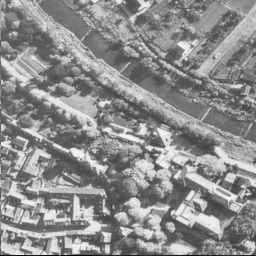
\includegraphics[width=0.95\textwidth]{figures/test-images/original/aerial}
  \caption{Aerial}
  \label{fig:test-images-aerial}
\end{subfigure}
\begin{subfigure}[b]{.3\textwidth}
  \centering
  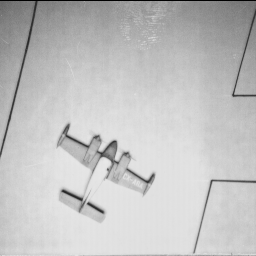
\includegraphics[width=0.95\textwidth]{figures/test-images/original/airplane}
  \caption{Airplane}
  \label{fig:test-images-airplane}
\end{subfigure}
\begin{subfigure}[b]{.3\textwidth}
  \centering
  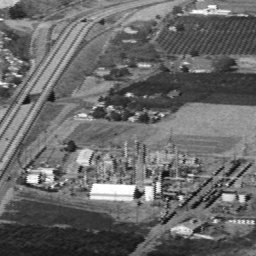
\includegraphics[width=0.95\textwidth]{figures/test-images/original/chemicalplant}
  \caption{Chemical plant }
  \label{fig:test-images-chemicalplant}
\end{subfigure}
\begin{subfigure}[b]{.3\textwidth}
  \centering
  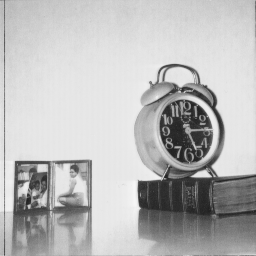
\includegraphics[width=0.95\textwidth]{figures/test-images/original/clock}
  \caption{Clock}
  \label{fig:test-images-clock}
\end{subfigure}
\begin{subfigure}[b]{.3\textwidth}
  \centering
  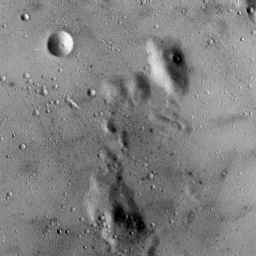
\includegraphics[width=0.95\textwidth]{figures/test-images/original/moonsurface}
  \caption{Moon surface}
  \label{fig:test-images-moonsurface}
\end{subfigure}
\begin{subfigure}[b]{.3\textwidth}
  \centering
  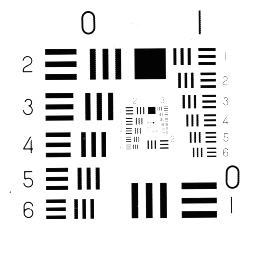
\includegraphics[width=0.95\textwidth]{figures/test-images/original/resolutionchart}
  \caption{Resolution chart}
  \label{fig:test-images-resolutionchart}
\end{subfigure}
\caption{256x256 pixel 8-bits grayscale test images \cite{USC:SIPI}}
\label{fig:test-images}
\end{figure}




\begin{figure}
\centering
\begin{subfigure}[b]{.23\textwidth}
  \centering
  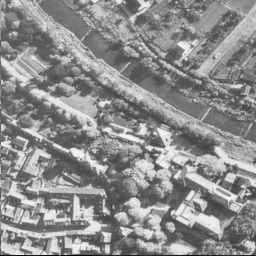
\includegraphics[width=0.95\textwidth]{figures/test-images/original/aerial}
  \caption{Aerial}
  \label{fig:test-images-aerial}
\end{subfigure}
\begin{subfigure}[b]{.23\textwidth}
  \centering
  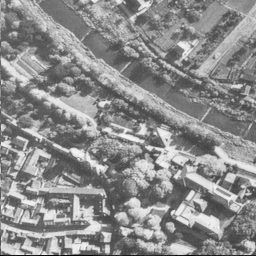
\includegraphics[width=0.95\textwidth]{figures/test-images/truncate1/aerial}
  \caption{}
  \label{fig:test-images-aerial}
\end{subfigure}
\begin{subfigure}[b]{.23\textwidth}
  \centering
  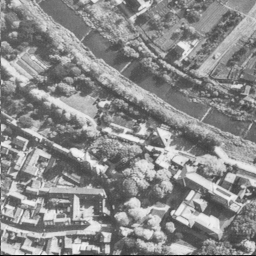
\includegraphics[width=0.95\textwidth]{figures/test-images/truncate2/aerial}
  \caption{}
  \label{fig:test-images-aerial}
\end{subfigure}
\begin{subfigure}[b]{.23\textwidth}
  \centering
  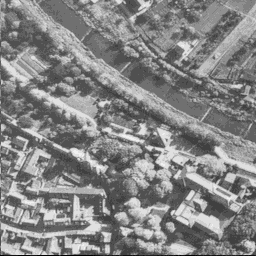
\includegraphics[width=0.95\textwidth]{figures/test-images/truncate4/aerial}
  \caption{}
  \label{fig:test-images-aerial}
\end{subfigure}

\begin{subfigure}[b]{.23\textwidth}
  \centering
  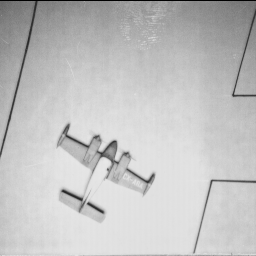
\includegraphics[width=0.95\textwidth]{figures/test-images/original/airplane}
  \caption{Airplane}
  \label{fig:test-images-airplane}
\end{subfigure}
\begin{subfigure}[b]{.23\textwidth}
  \centering
  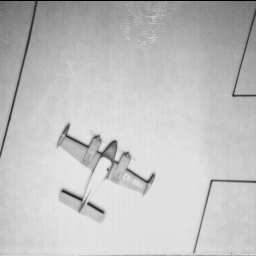
\includegraphics[width=0.95\textwidth]{figures/test-images/truncate1/airplane}
  \caption{}
  \label{fig:test-images-airplane}
\end{subfigure}
\begin{subfigure}[b]{.23\textwidth}
  \centering
  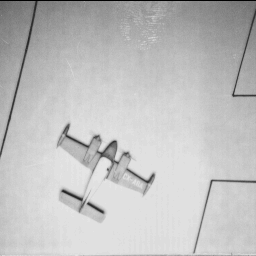
\includegraphics[width=0.95\textwidth]{figures/test-images/truncate2/airplane}
  \caption{}
  \label{fig:test-images-airplane}
\end{subfigure}
\begin{subfigure}[b]{.23\textwidth}
  \centering
  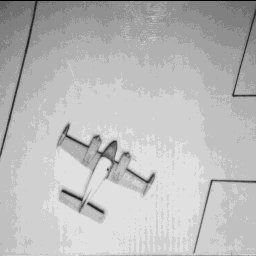
\includegraphics[width=0.95\textwidth]{figures/test-images/truncate4/airplane}
  \caption{}
  \label{fig:test-images-airplane}
\end{subfigure}

\begin{subfigure}[b]{.23\textwidth}
  \centering
  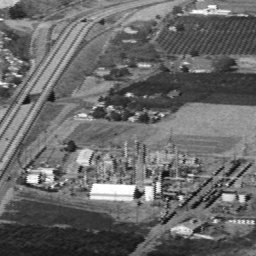
\includegraphics[width=0.95\textwidth]{figures/test-images/original/chemicalplant}
  \caption{Chemical plant}
  \label{fig:test-images-chemicalplant}
\end{subfigure}
\begin{subfigure}[b]{.23\textwidth}
  \centering
  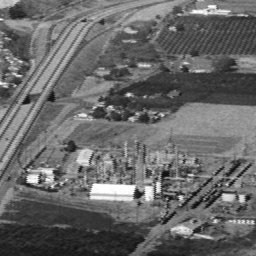
\includegraphics[width=0.95\textwidth]{figures/test-images/truncate1/chemicalplant}
  \caption{}
  \label{fig:test-images-chemicalplant}
\end{subfigure}
\begin{subfigure}[b]{.23\textwidth}
  \centering
  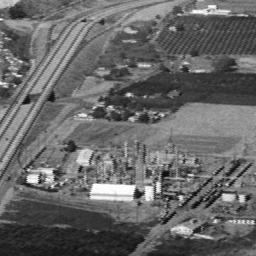
\includegraphics[width=0.95\textwidth]{figures/test-images/truncate2/chemicalplant}
  \caption{}
  \label{fig:test-images-chemicalplant}
\end{subfigure}
\begin{subfigure}[b]{.23\textwidth}
  \centering
  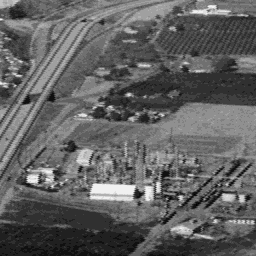
\includegraphics[width=0.95\textwidth]{figures/test-images/truncate4/chemicalplant}
  \caption{}
  \label{fig:test-images-chemicalplant}
\end{subfigure}

\begin{subfigure}[b]{.23\textwidth}
  \centering
  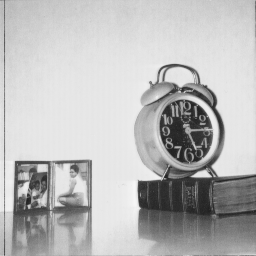
\includegraphics[width=0.95\textwidth]{figures/test-images/original/clock}
  \caption{Clock}
  \label{fig:test-images-clock}
\end{subfigure}
\begin{subfigure}[b]{.23\textwidth}
  \centering
  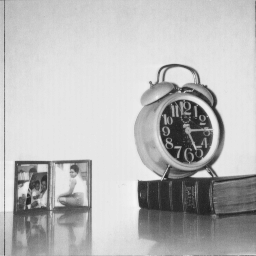
\includegraphics[width=0.95\textwidth]{figures/test-images/truncate1/clock}
  \caption{}
  \label{fig:test-images-clock}
\end{subfigure}
\begin{subfigure}[b]{.23\textwidth}
  \centering
  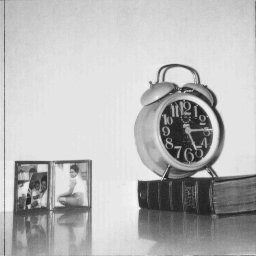
\includegraphics[width=0.95\textwidth]{figures/test-images/truncate2/clock}
  \caption{}
  \label{fig:test-images-clock}
\end{subfigure}
\begin{subfigure}[b]{.23\textwidth}
  \centering
  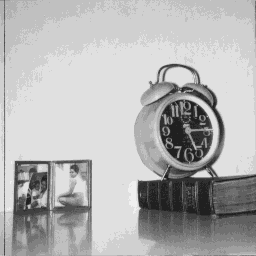
\includegraphics[width=0.95\textwidth]{figures/test-images/truncate4/clock}
  \caption{}
  \label{fig:test-images-clock}
\end{subfigure}

\begin{subfigure}[b]{.23\textwidth}
  \centering
  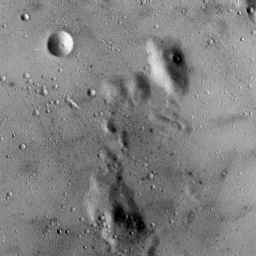
\includegraphics[width=0.95\textwidth]{figures/test-images/original/moonsurface}
  \caption{Moon surface}
  \label{fig:test-images-moonsurface}
\end{subfigure}
\begin{subfigure}[b]{.23\textwidth}
  \centering
  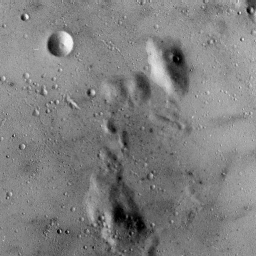
\includegraphics[width=0.95\textwidth]{figures/test-images/truncate1/moonsurface}
  \caption{}
  \label{fig:test-images-moonsurface}
\end{subfigure}
\begin{subfigure}[b]{.23\textwidth}
  \centering
  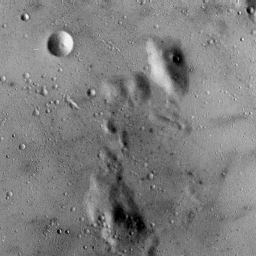
\includegraphics[width=0.95\textwidth]{figures/test-images/truncate2/moonsurface}
  \caption{}
  \label{fig:test-images-moonsurface}
\end{subfigure}
\begin{subfigure}[b]{.23\textwidth}
  \centering
  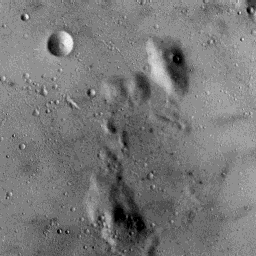
\includegraphics[width=0.95\textwidth]{figures/test-images/truncate4/moonsurface}
  \caption{}
  \label{fig:test-images-moonsurface}
\end{subfigure}

\begin{subfigure}[b]{.23\textwidth}
  \centering
  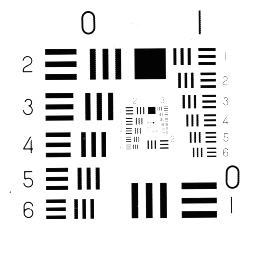
\includegraphics[width=0.95\textwidth]{figures/test-images/original/resolutionchart}
  \caption{Res. chart}
  \label{fig:test-images-resolutionchart}
\end{subfigure}
\begin{subfigure}[b]{.23\textwidth}
  \centering
  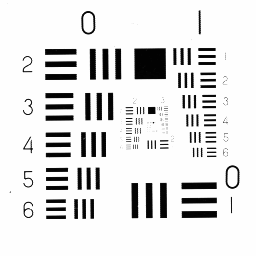
\includegraphics[width=0.95\textwidth]{figures/test-images/truncate1/resolutionchart}
  \caption{}
  \label{fig:test-images-resolutionchart}
\end{subfigure}
\begin{subfigure}[b]{.23\textwidth}
  \centering
  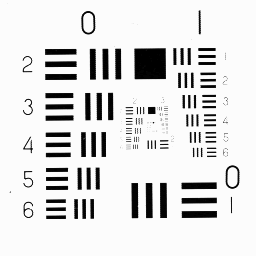
\includegraphics[width=0.95\textwidth]{figures/test-images/truncate2/resolutionchart}
  \caption{}
  \label{fig:test-images-resolutionchart}
\end{subfigure}
\begin{subfigure}[b]{.23\textwidth}
  \centering
  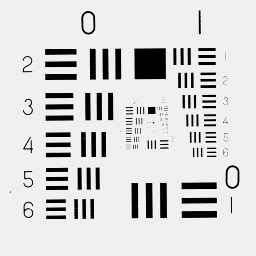
\includegraphics[width=0.95\textwidth]{figures/test-images/truncate4/resolutionchart}
  \caption{}
  \label{fig:test-images-resolutionchart}
\end{subfigure}

\caption{Restored images after lossy compression. Left picture is the original, right of it is the result of the Truncate1 compresseion, then Truncate2 and on the right Truncate4.}
\label{fig:test-images}
\end{figure}
